\section{Introduction}

One of the present challenges in cybersecurity systems is to outsource programs to be executed in the cloud and at the same time maintaining the privacy of the owner and the security of data. The program code has to be protected alongside the data which is being used inside it. Even in a securely encrypted code, the low-level instructions are visible when they are being executed by the CPU and a malicious operating system kernel can tamper with them. Several attacks are possible by reverse engineering the instructions, including code reuse, data injection, copyright violation, and recovery of classified data. Intel SGX (Software Guard eXtensions) \cite{sgx} is a novel architecture introduced with Intel Skylake micro-architecture \cite{skylake} that protects the code and the data inside an encrypted enclave that is a portion of memory which is protected by the support of hardware. The enclave is secure against direct eavesdropping by the adversary, but there are several successful attacking methods using side-channel information which is visible to the adversary \cite{leakycauldron}. The problem with this hardware extension is that the memory layout is still visible to the operating system kernel and a malicious OS in the cloud can recover useful information by observing the occurrences of page faults. As a result, this side-channel attack can be successful on recovering the data by clearing the page table and causing page faults and observing them for different inputs. In the same scenario, cache-misses are a point for side-channel attacks. The pattern of cache-miss occurrences can be used by a malicious operating system to attack the enclave program.

Several theoretical and practical attacks based on SGX side channels discussed and experimented to be practical and effective. The points of interest during the execution of a program inside enclave for the adversary are cache and whatever is missed and retrieved from the memory, page-faults, and page-table which is attacked by making use of accessed and modified bits.

In response to the development of attacks, several defense mechanisms are designed which have been effective in some cases and conditions. These defense methods usually sacrifice performance or accuracy while improving the security against side-channel attacks. 

In this report, we study the possible attacks which are possible using SGX side-channel information and their points of success. Then, we discuss possible defenses which have been proposed by the researchers and study their methods and compare the defenses and their effectiveness under different conditions and scenarios.

In summary, the main points of study in this work are:
\begin{itemize}
	\item Examining SGX enclave points of attacks.
	\item Discussing the past work which have been done on defending the SGX enclave against side-channel attacks.
	\item Comparing and analyzing the defense methods and their effectiveness.
\end{itemize} 
\textbf{Outline} In the remainder of this report, we discuss basic background knowledge required for studying this work in section 2. Then, we review and analyze the attacks which are possible to be launched against SGX enclave using side-channel information in section 3. In section 4, we introduce several defenses which have been proposed by past researches and in section 5 we analyze and compare the effectiveness of these defense methods in terms of security and performance. At last, we conclude the research in section 6.
\section{Background}
In this section, we provide detailed background on side-channel attacks targeting enclaved applications, tools, and terms we use in this report.

\subsection{Intel SGX}

Protecting the data inside a shield has been a major interest for improving security and privacy in distributed systems and several software-based and hardware-based solutions have been proposed for this purpose.

Intel introduced a new hardware-based technique in its new Skylake micro-architecture \cite{skylake} line of processors called Software Guard eXtensions (SGX) \cite{sgx}. The main function of it is assigning a portion of main memory to a program and protect it from being read and written by other processes. The effectiveness of this technique scales up to preventing the operating system kernel itself from accessing the shielded memory which is called enclave. Intel SGX API \cite{sgxapi} uses two main kinds of specialized function calls to work with enclave. ECALLs are functions which run inside the enclave and can be called from outside and OCALLs are useful for using system functions and other operations which are possible to be done outside enclave \cite{ecallocall}.

One of the major problems with running applications inside the cloud is the leakage of data and code instructions. Even with encryption, the CPU can only execute unencrypted instructions which can be eavesdropped and reverse engineered to useful code. Only with hardware modifications and adding SGX support to the hardware, it is possible to improve security and privacy in this term.

\subsection{Storage Structure}

In the common hardware architectures used in cloud computing environments today, data is transferred through several buses using multiple protocols to be used. The encrypted data is stored on the hard drive and will be transferred into enclaved memory. The encrypted data in the main memory will be cached using multiple levels of cache for performance optimization. Also, page mappings between virtual and physical addresses of data are kept in the main memory and a transaction look-aside buffer (TLB) is used to cache the mappings in the page-table for better performance.

Each data transfer can be a point of side-channel attack. While the data is encrypted, the patterns of reads and writes, cache-misses, page-faults, and other interrupts and exceptions can be used by the adversary for launching attacks and recovering useful information.

\subsection{Side-Channel Attacks on the Enclave}

Multiple effective attacks and defenses on the enclave have been proposed by past research. Most of the attacks make use of the side-channel information that can be leaked and accessed by a modified malicious kernel. In these attacks, the malicious kernel retrieves useful information about the code and the data by changing the behavior of program execution or analyzing the page-faults and other possible points of data leakage.

One of the major points of attacks is targeting exceptions caused by the program. Since the exceptions are first acknowledged by the kernel before the program, a malicious OS can use them to infer activities and the behavior of the program according to the inputs which leads to recovering the actual data and code of the program.

Another kind of attack that can be triggered by a malicious OS is an interrupt-based attack. The kernel can trigger interrupts to control the execution of the program.

Other attacks such as Stealthy Page Monitoring (SPM) attacks \cite{telling,leakycauldron} can also be effective. For a typical page-fault attack, the attacker can make all the page table entries invalid and restrict enclave program’s access to all the pages and by causing page-faults, view the pattern of memory reads and writes by the program. This action will cause a lot of page-faults which lead to a high overhead which leads to attack detection by the victim, so the attacker is interested to retrieve this information and view the pattern without causing unwanted page-faults by the victim. In page monitoring attacks, the attacker monitors the bits representing the validity and whether a page is accessed or modified. The attacker is also able to clear these bits and view them again frequently. So, the pattern of accesses can be visible to the attacker without causing page-faults \cite{telling,leakycauldron}.

\subsection{Intel TSX}
One of the technologies which have been came into notice for making benefit in defense against side-channel attacks is Intel TSX \cite{tsx}. This technology has been introduced by Intel since Haswell mirco-architecture \cite{haswell} for critical sections management and monitoring serialization. Intel TSX provides two frameworks to add transaction support to the processor. Both frameworks intoduce new instructions for region specification, backward compatiblity, and flexiblity \cite{tsx}. We use RTM (Restricted Transactional Memory) \cite{rtm} for implementing our defenses in this work.

RTM has been used by previous researches like T-SGX \cite{tsgx} to isolate instructions and Cloak \cite{cloak} to pin sensitive code and data to the caches which is not supported by current hardware instructions.

%We use RTM transactions to detect attacks against the executing program inside enclave. By using RTM, we detect page-faults, interrupts and other unusual behavior performed by the attacker and we can terminate if we guess we are being attacked.

\section{Attacks}

\section{Defenses}
% Head 1
\section{MMSN Protocol}

% Head 2
\subsection{Frequency Assignment}

We propose a suboptimal distribution to be used by each node, which is
easy to compute and does not depend on the number of competing
nodes. A natural candidate is an increasing geometric sequence, in
which
% Numbered Equation
\begin{equation}
\label{eqn:01}
P(t)=\frac{b^{\frac{t+1}{T+1}}-b^{\frac{t}{T+1}}}{b-1},
\end{equation}
where $t=0,{\ldots}\,,T$, and $b$ is a number greater than $1$.

In our algorithm, we use the suboptimal approach for simplicity and
generality. We need to make the distribution of the selected back-off
time slice at each node conform to what is shown in
Equation~\eqref{eqn:01}. It is implemented as follows: First, a random
variable $\alpha$ with a uniform distribution within the interval $(0,
1)$ is generated on each node, then time slice $i$ is selected
according to the following equation:
% Unnumbered Equation
\[
i=\lfloor(T+1)\log_b[\alpha(b-1)+1]\rfloor.
\]
It can be easily proven that the distribution of $i$ conforms to Equation
(\ref{eqn:01}).

So protocols \cite{Bahl-02, Culler-01,Zhou-06,Adya-01,
Tzamaloukas-01, Akyildiz-01} that use RTS/CTS
controls\footnote{RTS/CTS controls are required to be implemented by
802.11-compliant devices. They can be used as an optional mechanism
to avoid Hidden Terminal Problems in the 802.11 standard and
protocols based on those similar to \cite{Akyildiz-01} and
\cite{Adya-01}.} for frequency negotiation and reservation are not
suitable for WSN applications, even though they exhibit good
performance in general wireless ad-hoc
networks.

% Head 3
\subsubsection{Exclusive Frequency Assignment}


In exclusive frequency assignment, nodes first exchange their IDs
among two communication hops so that each node knows its two-hop
neighbors' IDs. In the second broadcast, each node beacons all
neighbors' IDs it has collected during the first broadcast period.

% Head 4
\paragraph{Eavesdropping}

Even though the even selection scheme leads to even sharing of
available frequencies among any two-hop neighborhood, it involves a
number of two-hop broadcasts. To reduce the communication cost, we
propose a lightweight eavesdropping scheme.

\subsection{Basic Notations}

As Algorithm~\ref{alg:one} states, for each frequency
number, each node calculates a random number (${\textit{Rnd}}_{\alpha}$) for
itself and a random number (${\textit{Rnd}}_{\beta}$) for each of its two-hop
neighbors with the same pseudorandom number generator.

% Algorithm
\begin{algorithm}[t]
\SetAlgoNoLine
\KwIn{Node $\alpha$'s ID ($ID_{\alpha}$), and node $\alpha$'s
neighbors' IDs within two communication hops.}
\KwOut{The frequency number ($FreNum_{\alpha}$) node $\alpha$ gets assigned.}
$index$ = 0; $FreNum_{\alpha}$ = -1\;
\Repeat{$FreNum_{\alpha} > -1$}{
        $Rnd_{\alpha}$ = Random($ID_{\alpha}$, $index$)\;
        $Found$ = $TRUE$\;
        \For{each node $\beta$ in $\alpha$'s two communication hops
    }{
      $Rnd_{\beta}$ = Random($ID_{\beta}$, $index$)\;
      \If{($Rnd_{\alpha} < Rnd_{\beta}$) \text{or} ($Rnd_{\alpha}$ ==
          $Rnd_{\beta}$ \text{and} $ID_{\alpha} < ID_{\beta}$)\;
      }{
        $Found$ = $FALSE$; break\;
      }
        }
     \eIf{$Found$}{
           $FreNum_{\alpha}$ = $index$\;
         }{
           $index$ ++\;
     }
      }
\caption{Frequency Number Computation}
\label{alg:one}
\end{algorithm}


Bus masters are divided into two disjoint sets, $\mathcal{M}_{RT}$
and $\mathcal{M}_{NRT}$.
% description
\begin{description}
\item[RT Masters]
$\mathcal{M}_{RT}=\{ \vec{m}_{1},\dots,\vec{m}_{n}\}$ denotes the
$n$ RT masters issuing real-time constrained requests. To model the
current request issued by an $\vec{m}_{i}$ in $\mathcal{M}_{RT}$,
three parameters---the recurrence time $(r_i)$, the service cycle
$(c_i)$, and the relative deadline $(d_i)$---are used, with their
relationships.
\item[NRT Masters]
$\mathcal{M}_{NRT}=\{ \vec{m}_{n+1},\dots,\vec{m}_{n+m}\}$ is a set
of $m$ masters issuing nonreal-time constrained requests. In our
model, each $\vec{m}_{j}$ in $\mathcal{M}_{NRT}$ needs only one
parameter, the service cycle, to model the current request it
issues.
\end{description}

Here, a question may arise, since each node has a global ID. Why
don't we just map nodes' IDs within two hops into a group of
frequency numbers and assign those numbers to all nodes within two
hops?

\section{Simulator}
\label{sec:sim}

If the model checker requests successors of a state which are not
created yet, the state space uses the simulator to create the
successors on-the-fly. To create successor states the simulator
conducts the following steps.
% enumerate
\begin{enumerate}
\item Load state into microcontroller model.
\item Determine assignments needed for resolving nondeterminism.
\item For each assignment.
      \begin{enumerate}
      \item either call interrupt handler or simulate effect of next instruction, or
      \item evaluate truth values of atomic propositions.
      \end{enumerate}
\item Return resulting states.
\end{enumerate}
Figure~\ref{fig:one} shows a typical microcontroller C program that
controls an automotive power window lift. The program is one of the
programs used in the case study described in Section~\ref{sec:sim}.
At first sight, the programs looks like an ANSI~C program. It
contains function calls, assignments, if clauses, and while loops.
% Figure
\begin{figure}
  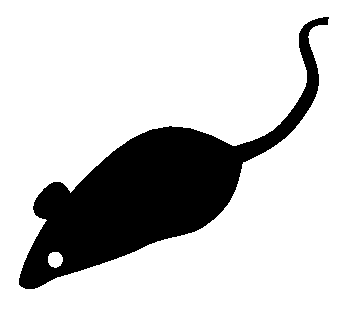
\includegraphics{mouse}
  \caption{Code before preprocessing.}
  \label{fig:one}
\end{figure}

\subsection{Problem Formulation}

The objective of variable coalescence-based offset assignment is to find
both the coalescence scheme and the MWPC on the coalesced graph. We start
with a few definitions and lemmas for variable coalescence.

% Enunciations
\begin{definition}[Coalesced Node (C-Node)]A C-node is a set of
live ranges (webs) in the AG or IG that are coalesced. Nodes within the same
C-node cannot interfere with each other on the IG. Before any coalescing is
done, each live range is a C-node by itself.
\end{definition}

\begin{definition}[C-AG (Coalesced Access Graph)]The C-AG is the access
graph after node coalescence, which is composed of all C-nodes and C-edges.
\end{definition}

\begin{lemma}
The C-MWPC problem is NP-complete.
\end{lemma}
\begin{proof} C-MWPC can be easily reduced to the MWPC problem assuming a
coalescence graph without any edge or a fully connected interference graph.
Therefore, each C-node is an uncoalesced live range after value separation
and C-PC is equivalent to PC. A fully connected interference graph is made
possible when all live ranges interfere with each other. Thus, the C-MWPC
problem is NP-complete.
\end{proof}

\begin{lemma}[Lemma Subhead]The solution to the C-MWPC problem is no
worse than the solution to the MWPC.
\end{lemma}
\begin{proof}
Simply, any solution to the MWPC is also a solution to the
C-MWPC. But some solutions to C-MWPC may not apply to the MWPC (if any
coalescing were made).
\end{proof}

\section{Performance Evaluation}

During all the experiments, the Geographic Forwarding (GF) by Akyildiz
et al.~\shortcite{Akyildiz-01} routing protocol is used. GF exploits
geographic information of nodes and conducts local data-forwarding to
achieve end-to-end routing. Our simulation is configured according to
the settings in Table~\ref{tab:one}. Each run lasts for 2 minutes and
repeated 100 times. For each data value we present in the results, we
also give its 90\% confidence interval.

% Table
\begin{table}%
\caption{Simulation Configuration}
\label{tab:one}
\begin{minipage}{\columnwidth}
\begin{center}
\begin{tabular}{ll}
  \toprule
  TERRAIN\footnote{This is a table footnote. This is a
    table footnote. This is a table footnote.}   & (200m$\times$200m) Square\\
  Node Number     & 289\\
  Node Placement  & Uniform\\
  Application     & Many-to-Many/Gossip CBR Streams\\
  Payload Size    & 32 bytes\\
  Routing Layer   & GF\\
  MAC Layer       & CSMA/MMSN\\
  Radio Layer     & RADIO-ACCNOISE\\
  Radio Bandwidth & 250Kbps\\
  Radio Range     & 20m--45m\\
  \bottomrule
\end{tabular}
\end{center}
\bigskip\centering
\footnotesize\emph{Source:} This is a table
 sourcenote. This is a table sourcenote. This is a table
 sourcenote.

 \emph{Note:} This is a table footnote.
\end{minipage}
\end{table}%


\section{Conclusions}

In this article, we develop the first multifrequency MAC protocol for
WSN applications in which each device adopts a
single radio transceiver. The different MAC design requirements for
WSNs and general wireless ad-hoc networks are
compared, and a complete WSN multifrequency MAC design (MMSN) is
put forth. During the MMSN design, we analyze and evaluate different
choices for frequency assignments and also discuss the nonuniform
back-off algorithms for the slotted media access design.

% Start of "Sample References" section

\section{Typical References in New ACM Reference Format}
A paginated journal article \cite{Abril07}, an enumerated
journal article \cite{Cohen07}, a reference to an entire issue \cite{JCohen96},
a monograph (whole book) \cite{Kosiur01}, a monograph/whole book in a series (see 2a in spec. document)
\cite{Harel79}, a divisible-book such as an anthology or compilation \cite{Editor00}
followed by the same example, however we only output the series if the volume number is given
\cite{Editor00a} (so Editor00a's series should NOT be present since it has no vol. no.),
a chapter in a divisible book \cite{Spector90}, a chapter in a divisible book
in a series \cite{Douglass98}, a multi-volume work as book \cite{Knuth97},
an article in a proceedings (of a conference, symposium, workshop for example)
(paginated proceedings article) \cite{Andler79}, a proceedings article
with all possible elements \cite{Smith10}, an example of an enumerated
proceedings article \cite{VanGundy07},
an informally published work \cite{Harel78}, a doctoral dissertation \cite{Clarkson85},
a master's thesis: \cite{anisi03}, an online document / world wide web
resource \cite{Thornburg01, Ablamowicz07, Poker06}, a video game (Case 1) \cite{Obama08} and (Case 2) \cite{Novak03}
and \cite{Lee05} and (Case 3) a patent \cite{JoeScientist001},
work accepted for publication \cite{rous08}, 'YYYYb'-test for prolific author
\cite{SaeediMEJ10} and \cite{SaeediJETC10}. Other cites might contain
'duplicate' DOI and URLs (some SIAM articles) \cite{Kirschmer:2010:AEI:1958016.1958018}.
Boris / Barbara Beeton: multi-volume works as books
\cite{MR781536} and \cite{MR781537}.

A couple of citations with DOIs: \cite{2004:ITE:1009386.1010128,
  Kirschmer:2010:AEI:1958016.1958018}.

Online citations: \cite{TUGInstmem, Thornburg01, CTANacmart}.

% Appendix
\appendix
\section{Switching Times}

In this appendix, we measure the channel switching time of Micaz
\cite{CROSSBOW} sensor devices.  In our experiments, one mote
alternatingly switches between Channels~11 and~12. Every time after
the node switches to a channel, it sends out a packet immediately and
then changes to a new channel as soon as the transmission is finished.
We measure the number of packets the test mote can send in 10 seconds,
denoted as $N_{1}$. In contrast, we also measure the same value of the
test mote without switching channels, denoted as $N_{2}$. We calculate
the channel-switching time $s$ as
\begin{displaymath}%
s=\frac{10}{N_{1}}-\frac{10}{N_{2}}.
\end{displaymath}%
By repeating the experiments 100 times, we get the average
channel-switching time of Micaz motes: 24.3\,$\mu$s.

\section{Supplementary Materials}


\begin{printonly}
  See the supplementary materials in the online version
\end{printonly}

\begin{screenonly}
\subsection{This is an Example of Appendix Subsection Head}

Channel-switching time is measured as the time length it takes for
motes to successfully switch from one channel to another. This
parameter impacts the maximum network throughput, because motes
cannot receive or send any packet during this period of time, and it
also affects the efficiency of toggle snooping in MMSN, where motes
need to sense through channels rapidly.

By repeating experiments 100 times, we get the average
channel-switching time of Micaz motes: 24.3 $\mu$s. We then conduct
the same experiments with different Micaz motes, as well as
experiments with the transmitter switching from Channel 11 to other
channels. In both scenarios, the channel-switching time does not have
obvious changes. (In our experiments, all values are in the range of
23.6 $\mu$s to 24.9 $\mu$s.)

\subsection{Appendix Subsection Head}

The primary consumer of energy in WSNs is idle listening. The key to
reduce idle listening is executing low duty-cycle on nodes. Two
primary approaches are considered in controlling duty-cycles in the
MAC layer.

\end{screenonly}

\begin{acks}

The authors would like to thank Dr. Maura Turolla of Telecom
Italia for providing specifications about the application scenario.

The work is supported by the \grantsponsor{GS501100001809}{National
  Natural Science Foundation of
  China}{http://dx.doi.org/10.13039/501100001809} under Grant
No.:~\grantnum{GS501100001809}{61273304\_a}
and~\grantnum[http://www.nnsf.cn/youngscientists]{GS501100001809}{Young
  Scientists' Support Program}.


\end{acks}

% Bibliography
\bibliographystyle{ACM-Reference-Format}
\bibliography{sample-bibliography}
